% 
\section{Question 1}
\subsection{Modelling Bird Population Decline Due to Invasive Snakes}
% 
\paragraph{In the modeling of bird populations after snake invasion, I utilized \textbf{Formula 1}. This choice was made to satisfy the requirements specified in the problem statement, where the population starts decreasing gradually after the snake invasion, and then, over time, the bird population experiences a sharp decline. Additionally, the modeling process should also account for the principles of \textbf{population dynamics} (in the later stages, due to a reduced availability of birds for the snakes to prey on, the snake population would also decrease, resulting in a slowdown in the rate of decline of the bird population).}
% 
% 
\begin{equation}
    P(t)=\frac{A}{e^{kt^2}}
\end{equation}
% 
% 
% 
% 
\paragraph{Where:}
\begin{itemize}
    \item \textbf{P(t)} is the population of birds at time 't'
    \item \textbf{A}: Maximum capacity, representing the constant bird population before snake invasion.
    \item \textbf{k} is a constant that determines the rate of decline.
\end{itemize}
% 
% 
% 
% 
\paragraph{Here is a brief proof where I applied SymPy to differentiate Formula 1. The code is provided below, and the result is (I preset A=1000, k=0.1):}
\begin{equation}
    P'(t)=-200.0te^{-0.1t^2}
\end{equation}
% 
\begin{lstlisting}[style=pystyle]
import sympy

# Define symbolic variable
t = sympy.symbols('t')

# Define constants
# Define the maximum capacity A, the value of k, 
# and the invasion time
A = 1000
k = 0.1

# Define the function
P = A * sympy.exp(-k * t**2)

# Calculate the derivative with resympyect to t
P_derivative = sympy.diff(P, t)

# Print the elegant mathematical expression
P_derivative
\end{lstlisting}
% 
% 
% 
% 
\paragraph{After I computed the derivative of $P(t)$ using SymPy, I employed the Python library Matplotlib to create a graphical representation of the derivative (\textbf{Figure 1}). I found that it meets the specified criteria, with the derivative values always being less than or equal to 0. Initially, the derivative is far from the x-axis, indicating an increasing rate of decline, while in the later portion, it starts to exhibit a deceleration in the decline rate.}
% 
% 
% 
% 
% 
$$  $$
% 
% 
% 
% 
% 
% 
% 
\begin{figure}[H]
    \centering
    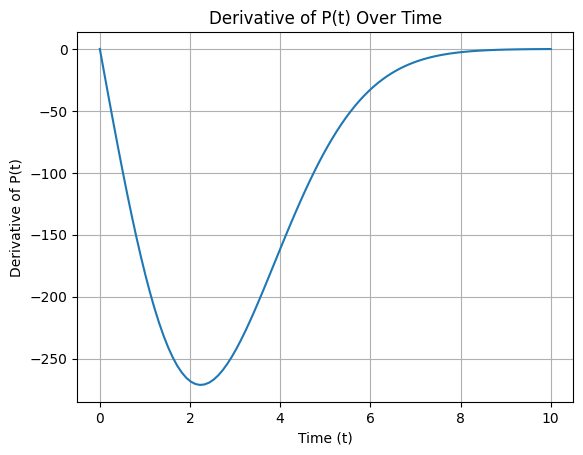
\includegraphics[width=0.7\textwidth]{pic/derivative_pt.png}
    \caption{Derivative of P(t)}
\end{figure}
% 
% 
% 
% 
% 
% 
% 
\paragraph{Finally, I took into account the event of snake invasion by introducing an invasion event. Before this event, the bird population remains constant.}
% 
$$  $$
% 
\begin{lstlisting}[style=pystyle]
# import numpy as np
# import matplotlib.pyplot as plt
import numpy as np

def bird_population_model(t, A, k, invade_time):
    P = np.zeros_like(t)  # Initialize the population array

    for i in range(len(t)):
        if t[i] < invade_time:
            P[i] = A  # Bird population remains constant before invasion
        else:
            P[i] = A * np.exp(-k * (t[i] - invade_time)**2)

    return P


invade_time = 5  # Time of snake invasion

# Generate a time range for plotting
t = np.linspace(0, 15, 100)  # Adjust the time range as needed

# Calculate the population over time
P = bird_population_model(t, A, k, invade_time)

# Plot the population over time
plt.plot(t, P)
plt.xlabel("Time")
plt.ylabel("Bird Population")
plt.title("Bird Population Over Time")
plt.grid(True)
plt.show()
\end{lstlisting}
% 
% 
% 
% 
% 
\paragraph{\textbf{Figure 2} represents the final graph I created.}
% 
% 
% BirdPopullationModel
\begin{figure}[H]
    \centering
    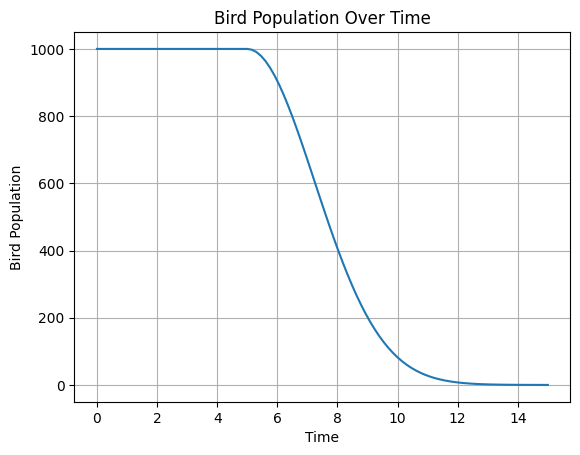
\includegraphics[width=0.75\textwidth]{pic/BirdPopullationModel.png}
    \caption{Figure of Bird Popullation Model}
\end{figure}
% 
% 
% 
% 
% 
% 
% 
% 
% 
% 
\subsection{Seasonal Epidemiological Models}
% 
% 
\paragraph{In this code, the abscissa shows the summer and winter of each year, with the number of cases increasing in the summer and remaining the same in the winter. To achieve this, we use the integer part to determine the year in order to switch between summer and winter. Custom labels were also created for the x-axis to represent the seasons of the year.}
% 
$$  $$
% 
% 
\begin{lstlisting}[style=pystyle]
import numpy as np
import matplotlib.pyplot as plt

def pandemic_model(t):
    # Define the peak year and the duration of the pandemic
    peak_year = 5
    duration = 10

    # Calculate the number of cases based on the given conditions
    cases = np.zeros_like(t)
    for i in range(len(t)):
        year = int(t[i])
        if 0 <= year < peak_year:
            cases[i] = (year + t[i] - year) / peak_year * (duration / 2)
        elif peak_year <= year < peak_year + duration / 2:
            cases[i] = (1 - (year + t[i] - year - peak_year) / (duration / 2)) * (duration / 2)

    return cases

# Generate a time range for plotting (a decade)
t = np.linspace(0, 10, 100)

# Calculate the number of cases over the decade
cases = pandemic_model(t)

# Create custom labels for x-axis to represent summer and winter
x_labels = [f'Year {int(year)} {"Summer" if int(year) % 1 == 0 else "Winter"}' for year in t]

# Plot the number of cases over time
plt.plot(x_labels, cases)
plt.xlabel("Time (Year and Season)")
plt.ylabel("Number of Cases")
plt.title("Pandemic Cases Over a Decade with Seasonal Variation")
plt.grid(True)
plt.xticks(rotation=45)
plt.show()
\end{lstlisting}
% 
% 
% 
% 
% 
% 
% 
% 
% 
% 
% 
\paragraph{The result of this code is \textbf{Figure 3}. The number of cases changes only when the Season is summer.}
% 
% 
% 
% 
% 
% 
% 
% 
% 
% 
% 
\begin{figure}[H]
    \centering
    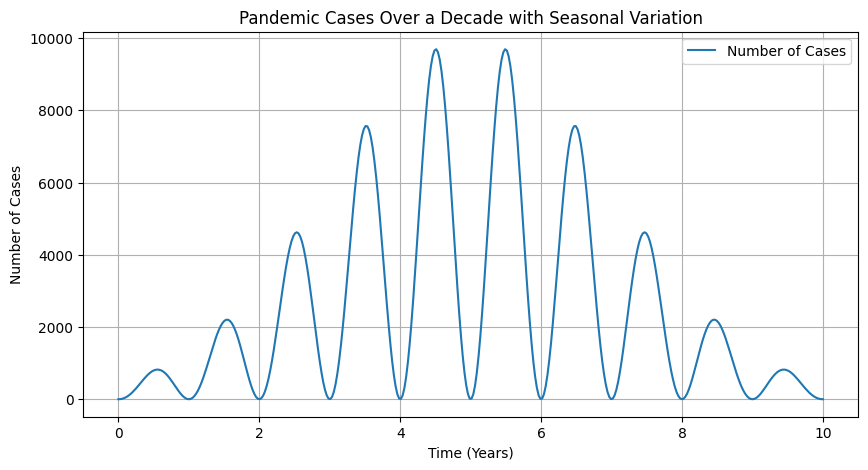
\includegraphics[width=0.85\textwidth]{pic/Pandemic_cases.png}
    \caption{Figure of Pandemic Cases}
\end{figure}
% 
% 
% 
% 
% 
% 
% 
% 
% 
% 